\documentclass[aspectratio=169]{beamer}
%\usetheme{Marburg}
\usepackage[utf8]{inputenc}
\usepackage[russian]{babel}
\usepackage[OT1]{fontenc}
\usepackage{amsmath}
\usepackage{amsfonts}
\usepackage{amssymb}
\usepackage{graphicx}
\usepackage{mathtools}
\usepackage{xcolor}
\usepackage{empheq}
\usepackage[many]{tcolorbox}
\usepackage{multirow}

\author{Николай Анохин}

\title{Краткое введение в data mining}
%\setbeamercovered{transparent} 
\setbeamertemplate{navigation symbols}{} 
%\logo{} 
%\institute{} 
\date{} 
%\subject{}

\tcbset{highlight math style={enhanced,colframe=red,colback=white,arc=4pt,boxrule=1pt}}

\begin{document}

\begin{frame}
\titlepage
\end{frame}

\section{Задача data mining}

\begin{frame}{Data Mining как KDD}

\begin{quote}{Knowledge Discovery in Databases (KDD)}
-- это процесс получения точных, неизвестных, потенциально полезных и интерпретируемых закономерностей из данных.\footnote{U. Fayyad, G. Piatetsky-Shapiro, P. Smyth. From data mining to knowledge discovery: an overview. 1996}
\end{quote}

\end{frame}

\begin{frame}{Data Mining как моделирование}

\begin{quote}{Data Mining}
-- процесс построения модели, хорошо описывающей закономерности, которые порождают данные.
\end{quote}

Подходы к построению моделей
\begin{itemize}
\item cтатистический
\item машинное обучение
\item вычислительный
\end{itemize}

\end{frame}

\begin{frame}
\frametitle<1>{Качество вина\footnote{\href{https://archive.ics.uci.edu/ml/datasets/Wine+Quality}{Wine Quality Data Set. UCI Machine Learning Repository}}}
\frametitle<2>{Качество вина: статистический подход}
\frametitle<3>{Качество вина: машинное обучение}
\frametitle<4>{Качество вина: вычислительный подход}

\begin{columns}[c]
    \begin{column}{.49\linewidth}
    \begin{footnotesize}
    \begin{overprint}
				\onslide<1>
				\begin{center}			
			\begin{tabular}{r  c  c}
			& ABV, \% & Quality \\
			\hline
			1 & 12.8 & good \\
			2 & 12.8 & good \\
			3 & 10.5 & good \\
			4 & 10.7 & good \\
			5 & 10.7 & good \\
			$\ldots$ & $\ldots$ & $\ldots$ \\
			198 & 11.4 & good \\
			199 & 10.10 & bad \\
			200 & 10.30 & bad \\
			201 & 10.90 & bad \\
			202 & 9.95 & bad \\
			$\ldots$ & $\ldots$ & $\ldots$ \\
			444 & 9.05 & bad \\
			\end{tabular}
			\end{center}
			  \onslide<2>
			  \[
			\begin{cases}
			p( \text{alcohol} \mid \text{good} ) \sim \mathcal{N}(\text{alcohol} \mid \mu_g, \sigma_g) \\
			p( \text{alcohol} \mid \text{bad} ) \sim \mathcal{N}(\text{alcohol} \mid \mu_b, \sigma_b) \\
			\end{cases}
			\]
			\[
			\qquad\qquad\Downarrow (\text{ML-принцип})
			\]
			\[
			\begin{cases} 
			\mu_g=11.4, \sigma_g=1.3 \\ 
			\mu_b=10.2, \sigma_b=1.0
			\end{cases}
			\]
			  \onslide<3> 
			  Обучаем линейный SVM: 
			  \[\text{alcohol} > 11.2 \Rightarrow \text{good}\]
			  \onslide<4>
			  Подсчитываем параметры данных: \[\langle \text{alcohol} \rangle_g = 11.4,\; \langle \text{alcohol} \rangle_b = 10.2\]		
		\end{overprint}
		\end{footnotesize}
    \end{column}    
    \begin{column}{.49\linewidth}
    \begin{center}
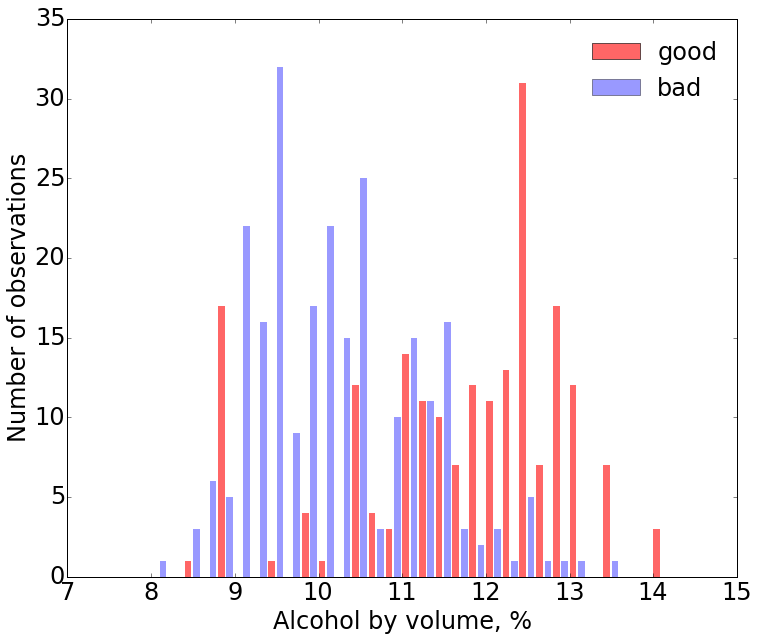
\includegraphics[width=0.95\textwidth]{images/wine.png}
\end{center}   
    \end{column}
\end{columns}

\end{frame}

\begin{frame}{Data Mining -- область на пересечении дисциплин\footnote{\href{http://blogs.sas.com/content/subconsciousmusings/2014/08/22/looking-backwards-looking-forwards-sas-data-mining-and-machine-learning/}{Looking backwards, looking forwards: SAS, data mining, and machine learning}}}

\begin{center}
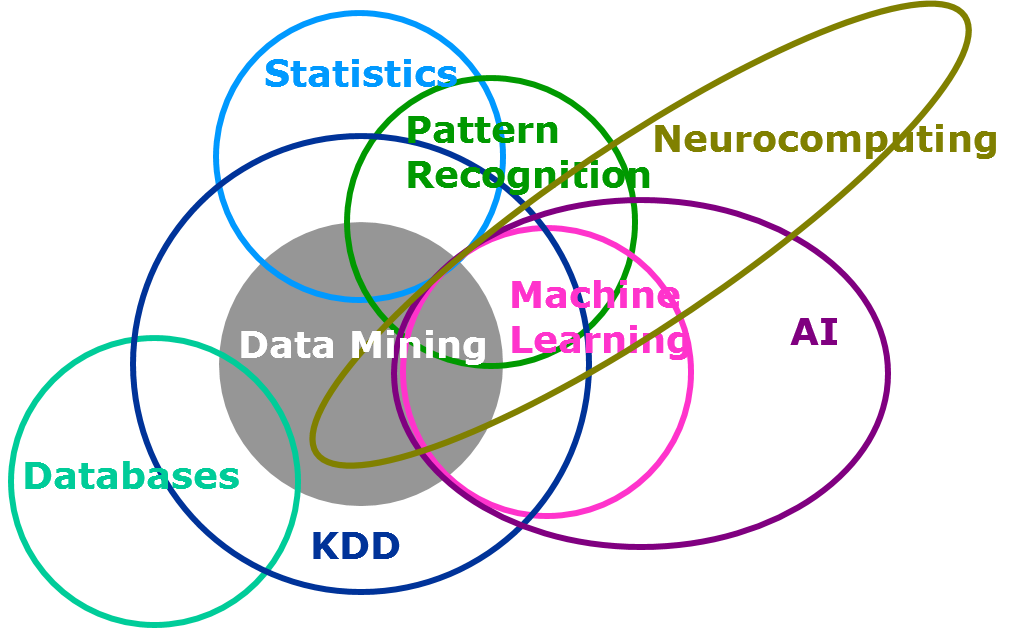
\includegraphics[width=0.75\textwidth]{images/data-mining-venn.png}
\end{center}

\end{frame}

\begin{frame}{Data Mining -- область тысячи имен}

\begin{enumerate}
\item[1960-е] Data Fishing, Data Dredging
\item[1980-е] Knowledge Discovery in Databases
\item[1990-е] Data Mining, Database mining\textsuperscript{TM}
\item[2000-е] Data Analytics, Data Science\footnote{\href{https://twitter.com/nivertech/status/180109930139893761}{Data Scientist is a Data Analyst who lives in California}}\footnote{\href{https://twitter.com/josh_wills/status/198093512149958656}{A data scientist is someone who is better at statistics than any software engineer and better at software engineering than any statistician.}}
\end{enumerate}

\end{frame}

\begin{frame}{Некоторые важные события в истории Data Mining}

\begin{enumerate}
\item[1989] IJCAI-89 Workshop on Knowledge Discovery in Databases 
\item[1995] ACM SIGKDD Conference on Knowledge Discovery and Data Mining
\item[2001] Leo Breiman's ``Statistical Modeling: The Two Cultures''
\item[2003] Программа Total Information Awareness
\item[2005] Doug Cutting и Mike Cafarella разработали пакет обработки данных Hadoop
\item[2007] Первый релиз библиотки scikit-learn
\item[2010] Заработал сайт Kaggle -- платформа для проведения соревнований по Data Science
\item[2012] Harvard Business Review публикует статью Data Scientist: The Sexiest Job of the 21st Century
\item[2013] Первая встреча сообщества Moscow Data Science\footnote{\url{http://www.meetup.com/Moscow-Data-Science/}} в московском офисе Mail.Ru Group
\end{enumerate}

\end{frame}

\end{document}